\section{Related work}

\todo[inline]{Opsummer hvad vi har haft af related work i rapporten of
inkluder det der ikke passede ind}

The groundwork of regular expression has been known for
decades. Current research is often focused generally; for
example to improve matching speeds, but there is also heavy activity
towards more specialized purposes, such as XML parsers, hardware based spam
detection or even such fields as biology where regular expressions are
often used to find patterns of amino acids. 

The intended aim of this particular project is towards the general
realm (the curios reader may wish to read \todo{cite-dig-selv} if they
are interested in special usages of regular expressions). For this
reason, the remainder of this section will therefore concentrate on
likewise general research.

\todo{blah blah om ting du ikke har snakket naermere om}


\subsection{Constructing NFAs}

It is possible to construct different NFAs accepting the same
language. These NFAs will have different properties. 

\todo[inline]{Find out other methods for constructing NFAs}

\subsection{Simulating NFAs}

\subsubsection{Frisch and Cardelli}

Frisch and Cardelli presents a way of simulating a NFA in their paper
\cite{2004:GreedyRegularExpressionMatching}. It works in two passes
over the input string. The first pass annotates the input string with
enough information to decide which branch to pick in alternations and
how many times to iterate a quantifier. This is done by reading the
input from right-to-left and working our way backwards in the NFA, the
visited states are annotated and stored with the input string. In the
second and main pass, where we read the input string left-to-right and
work our forwards in the NFA, these annotations are used to decide
which branch to take in an alternation and how many times to iterate a
star. This method is not suitable for a streaming regular expression
engine. The input string is read first from end-to-front and then from
front-to-end, this can not be done without storing the string.

\subsubsection{Backtracking}
Backtracking is a way of simulating a NFA. It is the method employed
by many programming languages and libraries, such as Perl and
PCRE. Compared to other methods, this has the advantage of allowing
backreferences, but it is also a worst-case exponential-time
algorithm. An example of a matching that exhibits worst-case behavior
is the regular expression \textsf{a?$^n$a$^n$} and the string
\textsl{a$^n$}, where superscripts denotes string repetition. This
example is also known from the article \cite{RussCox}.

A backtracking algorithm works depth-first. It has one active state
(\texttt{AS}) and a string pointer (\texttt{SP}) and a stack of
save-points. Every time we have to make a choice as to which
transition to take when traversing the NFA, we save the state so we
can later return and explore the alternate routes. Each save-point
consists of a state and a pointer to the string.

\begin{example}[Backtracking]
\begin{figure}
  \centering 
  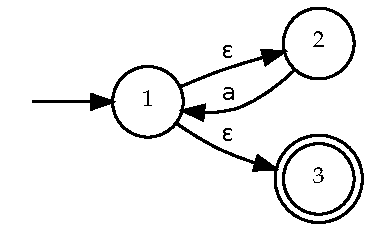
\includegraphics{relatedwork/backtracking.pdf}
  \caption{NFA for \textsf{a*}}
  \label{fig:backtracking}
\end{figure}
In this example we will be matching \textsf{a*} to the string
\textsl{aa}. The NFA we will be using for this example is in figure
\vref{fig:backtracking}. The process of matching could look like:
\begin{center}
\begin{tabular}{cccp{7.5cm}}
  \texttt{AS} & \texttt{SP} & Save-points & Explanation \\ 

  \hline 

  1 & \textsl{\underline{a}a} &
  \rowcolors[\hline]{1}{lightgray}{lightgray}
  \begin{tabular}{c}
    \\
  \end{tabular} 
  & Initially \texttt{AS} is set to the start state and \texttt{SP} is
  set to the first character in the string\\
  
  2 & \textsl{\underline{a}a} & 
  \rowcolors[\hline]{1}{lightgray}{lightgray}
  \begin{tabular}{c}
    (1, \textsl{\underline{a}a})\\
  \end{tabular} 
  & Two paths are available, so we save the state and take the
  $\upvarepsilon$-transition to state 2. \\

  1 & \textsl{a\underline{a}} & 
  \rowcolors[\hline]{1}{lightgray}{lightgray}
  \begin{tabular}{c}
    (1, \textsl{\underline{a}a})\\
  \end{tabular} 
  & We take the transition back to state 1 and consume the first
  \textsl{a}. \\

  2 & \textsl{a\underline{a}} & 
  \rowcolors[\hline]{1}{lightgray}{lightgray}
  \begin{tabular}{c}
    (1, \textsl{\underline{a}a}) \\
    (1, \textsl{a\underline{a}})\\
  \end{tabular} 
  & Two paths are available, so we save the state and take the
  $\upvarepsilon$-transition to state 2. \\
  
  1 & \textsl{aa\underline{ }} &
  \rowcolors[\hline]{1}{lightgray}{lightgray}
  \begin{tabular}{c}
    (1, \textsl{\underline{a}a}) \\
    (1, \textsl{a\underline{a}})\\
  \end{tabular} 
  & We take the transition back to state 1 and consume the second
  \textsl{a}. \\

  2 & \textsl{aa\underline{ }} & 
  \rowcolors[\hline]{1}{lightgray}{lightgray}
  \begin{tabular}{c}
    (1, \textsl{\underline{a}a}) \\
    (1, \textsl{a\underline{a}}) \\
    (1, \textsl{aa\underline{ }})
  \end{tabular} 
  & Two paths are available, so we save the state and take the
  $\upvarepsilon$-transition to state 2. \\
  
  \\

  1 & \textsl{\underline{a}a} &   
  \rowcolors[\hline]{1}{lightgray}{lightgray}
  \begin{tabular}{c}
    (1, \textsl{a\underline{a}}) \\
    (1, \textsl{aa\underline{ }})
  \end{tabular} 
  & No transitions are available from state 2, so this path is
  abandoned. We backtrack and pop a save-state. \\
  
  3 & \textsl{\underline{a}a} &   
  \rowcolors[\hline]{1}{lightgray}{lightgray}
  \begin{tabular}{c}
    (1, \textsl{a\underline{a}}) \\
    (1, \textsl{aa\underline{ }})
  \end{tabular} 
  & The other available $\upvarepsilon$-transition to state 3 is
  taken. \\

  1 & \textsl{a\underline{a}} &   
  \rowcolors[\hline]{1}{lightgray}{lightgray}
  \begin{tabular}{c}
    (1, \textsl{aa\underline{ }})
  \end{tabular} 
  & No transitions are available from state 3, so this path is
  abandoned. We backtrack and pop a save-state. \\
  
  3 & \textsl{a\underline{a}} &   
  \rowcolors[\hline]{1}{lightgray}{lightgray}
  \begin{tabular}{c}
    (1, \textsl{aa\underline{ }})
  \end{tabular} 
  & The other available $\upvarepsilon$-transition to state 3 is
  taken. \\

  1 & \textsl{aa\underline{}} &
  \rowcolors[\hline]{1}{lightgray}{lightgray}
  \begin{tabular}{c}
    \\
  \end{tabular} 
  & No transitions are available from state 3, so this path is
  abandoned. We backtrack and pop a save-state. \\

  
  3 & \textsl{a\underline{a}} &
  \rowcolors[\hline]{1}{lightgray}{lightgray}
  \begin{tabular}{c}
    \\
  \end{tabular} 
  & The other available $\upvarepsilon$-transition to state 3 is
  taken. We have reached the end of the string and are in an accepting
  state: We have a match! \\
\end{tabular}
\end{center}
\end{example}


\subsection{Virtual machine}
Another popular method of matching regular expressions to text is the
virtual machine approach \cite{Cox2009}. Instead of constructing a
automaton, we generate bytecode for an interpreter. 

A simple virtual machine would have the ability to execute threads,
each thread consisting of a regular expression program. Each thread
would maintain a program counter (\texttt{PC}) and a string pointer
(\texttt{SP}). A regular expression program could for example consist of
the following instructions:
\begin{description}
\item[\texttt{char} $c$] If the \texttt{SP} does not point to a $c$
  character, then this thread of execution is abandoned. Otherwise,
  the \texttt{SP} and the \texttt{PC} is advanced.
\item[\texttt{match}] Stop thread, we have a match.
\item[\texttt{jmp} $x$] \texttt{PC} is set to $x$.
\item[\texttt{split} $x$\texttt{,} $y$] Split the thread of execution. The new
  threads \texttt{PC} is set to $x$ and the old threads \texttt{PC} is
  set to $y$.
\end{description}
With these few and simple instructions we are able to compile regular
expressions with concatenation, alternation and repetition, see table
\vref{tab:code_sequences}. 
\ctable[
  caption = Code sequences,
  label = tab:code_sequences
]
{lll}
{}
{\FL
$a$       &              & \texttt{char} $a$ \ML
$e_1e_2$  &              & \textit{codes for $e_1$} \NN
          &              & \textit{codes for $e_2$} \ML
$e_1|e_2$ &              & \texttt{split L1, L2}\NN
          & \texttt{L1:} & \textit{codes for $e_1$} \NN
          &              & \texttt{jmp L3} \NN
          & \texttt{L2:} & \textit{codes for $e_2$} \NN
          & \texttt{L3:} & \ML
$e*$      & \texttt{L1:} & \texttt{split L2, L3}\NN
          & \texttt{L2:} & \textit{codes for $e$} \NN
          &              & \texttt{jmp L1} \NN
          & \texttt{L3:} & \LL
}

\begin{example}[Virtual machine]
We are now ready for a small example match, we can match the regular
expression \textsf{a*} with the string \textsl{aa}. The regular
expressions compiles to
\begin{verbatim}
0 split 1, 4
1 char a
2 jmp 0
4 match
\end{verbatim}
Running this on a virtual machine could look like
\begin{center}
\begin{tabular}{cccp{7.5cm}}
Thread & \texttt{PC} & \texttt{SP} & Explanation \\
\hline
%T1 & 0 & \textsl{\underline{a}a} & character matches \\
T1 & 0 & \textsl{\underline{a}a} & Create thread T2 with \texttt{PC}
set to 4 and \texttt{SP} at \textsl{\underline{a}a}. T1 continues
execution at 1. \\

T1 & 1 & \textsl{\underline{a}a} & Character matches, \texttt{SP} and
\texttt{PC} is advanced. \\

T1 & 2 & \textsl{a\underline{a}} & \texttt{PC} is set to 0.\\ 

T1 & 0 & \textsl{a\underline{a}} & Create thread T3 with \texttt{PC}
set to 4 and \texttt{SP} at \textsl{a\underline{a}}. T1 continues
execution at 1. \\

T1 & 1 & \textsl{a\underline{a}} & Character matches, \texttt{SP} and
\texttt{PC} is advanced. \\

T1 & 2 & \textsl{a\underline{a}} & \texttt{PC} is set to 0.\\

T1 & 0 & \textsl{aa\underline{ }} & Create thread T4 with \texttt{PC}
set to 4 and \texttt{SP} at \textsl{aa\underline{ }}. T1 continues
execution at 1. \\

T1 & 1 & \textsl{aa\underline{ }} & Character does not match and this
thread is abandoned.\\

T2 & 4 & \textsl{\underline{a}a} & We have a match. \\

T3 & 4 & \textsl{a\underline{a}} & We have a match. \\

T4 & 4 & \textsl{aa\underline{ }} & We have a match. \\
\end{tabular}
\end{center}
\end{example}

We believe this is how Perl matches \cite{pelreguts}. Running the
program with debug mode on makes Perl print a textual representation
of the bytecode the regular expression is compiled into. In section
\vref{sec:regexmach.pl} we have a small Perl experiment demonstrating
this feature. The results of running the program:
\begin{verbatim}
$ ./regexmach.pl 
Compiling REx "a*"
Final program:
   1: STAR (4)
   2:   EXACT <a> (0)
   4: END (0)
minlen 0 
Freeing REx: "a*"
\end{verbatim}

